% ACIIDS 2027 submission (Springer LNCS/LNAI style).
% Compile with the official Springer class: put llncs.cls and splncs04.bst
% (from https://www.springernature.com/gp/computer-science/lncs/conference-proceedings-guidelines
% or Overleaf's "Springer LNCS" template) in this folder, then:
%   pdflatex main; bibtex main; pdflatex main; pdflatex main
\documentclass[runningheads]{llncs}
\usepackage[T1]{fontenc}
\usepackage[utf8]{inputenc}
\usepackage{amsmath,amssymb,booktabs,array,graphicx}
\usepackage{microtype}
\usepackage{xcolor}
\usepackage{url}
\renewcommand\UrlFont{\color{black}\rmfamily}
\newcommand{\repourl}{\url{https://github.com/Baole13/bahnar-vietnamese-candidate-normalization}}
\begin{document}
\title{When Does Candidate Normalization Help? A Low-Resource Bahnar--Vietnamese Sentence Retrieval Study}
\titlerunning{Candidate Normalization for Bahnar--Vietnamese Retrieval}
% Fill in before submission. Check the ACIIDS 2027 call on whether review is anonymous.
\author{First Author\inst{1}\orcidID{0000-0000-0000-0000}}
\authorrunning{F. Author}
\institute{Affiliation, City, Country\\\email{author@example.org}}
\maketitle
\begin{abstract}
We study inference-time candidate-density normalization for Bahnar-to-Vietnamese sentence retrieval on BA48, a journalistic, silver-aligned benchmark (781 held-out queries, 780 candidates, 20 document families). A locked fusion of a Dice translation table, character TF--IDF and a neural bi-encoder reaches 739/781 strict Recall@1. A pre-specified CSLS-style correction whose candidate-density term is estimated from 3,327 \emph{training} queries raises this to 749/781 (14 corrections, four regressions; exact McNemar $p=0.031$; family-bootstrap 95\% interval $[+0.12,+2.44]$ points), and points the same way on a separate 768-query validation split. Train-derived corrections are stable when the number of evaluated queries shrinks, whereas transductive Sinkhorn balancing falls from 98.6\% to 94.7\% at 10\% query coverage. A train-derived Inverted Softmax whose temperature is chosen on validation scores higher (759/781) but is sharply peaked in that temperature, and it was added after test access. A blinded check by two Bahnar native speakers agrees with the silver labels on 17 of 18 discordant queries and on 60 of 60 random controls. A same-pool IBM1 baseline and a cross-corpus overlap audit clarify the lexical alternatives and data-independence limits. The contribution is a controlled empirical analysis of established normalizations, not a new algorithm or a claim of semantic gold accuracy.
\keywords{Bahnar \and Cross-lingual sentence retrieval \and Low-resource languages \and Hubness \and CSLS \and Evaluation validity.}
\end{abstract}
\section{Introduction}
Cross-lingual sentence retrieval finds an existing translation instead of generating one. For low-resource languages it supports bilingual corpus curation, translation-memory lookup and the evaluation of multilingual sentence representations \cite{artetxe2019margin}. Accuracy depends not only on the encoder but also on the \emph{inference-time scoring rule}: some target sentences receive high scores from many unrelated queries, and candidate-side density adjustment such as Cross-domain Similarity Local Scaling (CSLS) and Inverted Softmax changes the ranking \cite{dinu2015improving,smith2017offline,conneau2018word}.

A practical distinction is easy to overlook: \emph{where the density estimate comes from}. With a fixed Vietnamese index and Bahnar queries arriving one at a time, candidate-side statistics can be precomputed from a reference set of \emph{training} queries. A transductive method instead estimates them from the unlabeled queries being evaluated together. The two use different information, and a strong result on an almost one-to-one, full evaluation batch need not carry over to smaller or irregular batches. This matters for low-resource systems, whose reference data are small and whose deployment patterns are irregular.

We study this question for Bahnar--Vietnamese on BA48, a journalistic, automatically aligned parallel-sentence collection (781 Bahnar queries, 780 Vietnamese candidates, 20 document families in the held-out test). A Dice lexical table, character TF--IDF and a task-adapted multilingual encoder are held fixed. Our findings are:
\begin{enumerate}
\item \textbf{A train-derived correction gives a small, measurable gain.} A pre-specified CSLS-style correction ($k=3$) estimated from training queries raises strict Recall@1 from 739/781 to 749/781 (+1.28 points; 14 queries corrected, four regress; exact McNemar $p=0.031$). The same direction appears on a separate 768-query validation split (725$\to$734).
\item \textbf{Train-derived corrections are batch-stable; transductive Sinkhorn is not.} Sinkhorn reaches 98.59\% on the full batch but 94.67\% when only 10\% of the queries are present, while the train-derived rules stay flat (Fig.~\ref{fig:subsample}).
\item \textbf{A train-derived Inverted Softmax with a validation-selected temperature is stronger.} Validation picks $\beta=2$, which reaches 759/781 on the test (20 corrections, none lost), but accuracy is sharply peaked: at $\beta=5$ it is no better than the baseline (741 vs.\ 739) and at $\beta=10$ it is worse (735). The method was first examined after test access, so it is a validation-selected secondary result, not the pre-specified one.
\item \textbf{A blinded check by two Bahnar native speakers broadly supports the silver labels} on the discordant queries and on 60 random controls (Section~\ref{sec:human}).
\end{enumerate}
We neither introduce CSLS nor claim state-of-the-art Bahnar retrieval; the contribution is a controlled, audited comparison of established normalizations under explicit assumptions about what information is available at inference time. The audits also expose remaining uncertainties: silver references, historical source reuse and archival encoder provenance.

\section{Related Work}
\paragraph{Cross-lingual ranking and normalization.} Globally corrected retrieval and Inverted Softmax reduce hubness in mapped spaces \cite{dinu2015improving,smith2017offline}; CSLS corrects for local neighbourhood densities \cite{conneau2018word}. Ratio-margin scores are used in multilingual bitext mining \cite{artetxe2019margin}. Sinkhorn balancing comes from entropy-regularized optimal transport \cite{cuturi2013sinkhorn}. These are \emph{established} methods; our question is how their evaluation depends on training-reference statistics versus an unlabeled query batch, with the scorer held constant.

\paragraph{Bahnar retrieval and language resources.} Prior work combines dictionaries and neural models for Vietnamese--Bahnar translation \cite{vo2024revitalizing,nguyen2025bartbahnar}, and sentence-aware bilingual lexical mapping has been studied \cite{nguyen2026sentenceaware}. Most directly, Nguyen et al.~\cite{nguyen2026parallelretrieval} compare lexical, IBM Model~1 (IBM1), dense and hybrid Bahnar--Vietnamese retrieval on a separate 2,001-pair test with a 2,001-candidate pool, report 0.4933 R@1 for symmetric IBM1 and 0.5162 for their best reranker, and also evaluate CSLS and ratio margin with $k=10$. As described there, the neighbourhood means are computed over the full query set and candidate pool before ranking; the neighbourhood statistics therefore come from the evaluated batch, which is the transductive setting we contrast with a train-derived reference. The two studies differ in corpus (a larger resource whose Bahnar text was checked by native speakers versus BA48 journalism), pool size, supervision and aim, so their numbers are not comparable. We use their publicly documented IBM1 configuration only as a clearly marked retrospective baseline on the BA48 pool.

\paragraph{Low-resource evaluation validity.} Translationese and a single designated counterpart can distort retrieval evaluation \cite{ni2022original,fomicheva2020multi}, and Bahnar varieties differ linguistically \cite{dinh2026registers}. We therefore report strict reference accuracy as a property of the observed written corpus, audit text overlap separately from semantic equivalence, and add a small native-speaker check.

\section{Data and Evaluation Integrity}\label{sec:data}
\paragraph{BA48.} BA48 contains 5,094 automatically aligned Vietnamese--Bahnar sentence pairs associated with 170 \emph{Bao anh Gia Lai} PDF URLs in the Bao Gia Lai archive \cite{baogialai2023thousand,baogialai2012translation}. The publication describes translating Vietnamese journalism into Bahnar; the evaluated retrieval direction is Bahnar query $\rightarrow$ Vietnamese candidate, against that presumed editorial direction. The corpus does not identify dialects for individual texts. The source flags indicate legacy-font decoding and automatic alignment, but the original conversion map, alignment software and item-level human quality-control decisions could not be recovered. Thus all train, validation and test labels are \emph{silver}, not adjudicated gold.

\begin{table}[t]
\centering\small
\caption{BA48 evaluation partitions. Families are connected components in a cross-PDF near-duplicate graph, not editorial article labels.}
\label{tab:splits}

\begin{tabular}{lrrr}
\toprule
Split & Sentence pairs & Families & PDFs \\
\midrule
Train (after quarantine) & 3,327 & 69 & 119 \\
Validation & 768 & 18 & 25 \\
Test & 781 & 20 & 26 \\
\bottomrule
\end{tabular}
\end{table}

BA48 was partitioned by near-duplicate-connected PDF families (107 components over 170 PDFs); the largest contains 51 PDFs. The training reservoir had 3,545 rows, from which 218 were quarantined for near-overlap with held-out material or a reserved source holdout. Validation and test were unchanged. The candidate pool consists of \emph{780 unique} Vietnamese test strings: two Bahnar queries share the same designated candidate. All evaluation operations use explicit query and candidate identifiers, not row-diagonal indices. The original fixed-pool setting assumes every query has a designated candidate and does not test no-match retrieval.

\paragraph{Distinct fitting sources.} Dice and character TF--IDF are fitted exclusively on a historical file of 55,324 unique parallel pairs. The E1 multilingual encoder had instead been trained on 50,283 historical auxiliary pairs plus the 3,327 BA48 adaptation-training pairs (53,610 total), with validation used for checkpoint selection. The 50,283 auxiliary pairs are a subset of the historical file. The fact that BA48 training is included in E1 makes E1's training-query scores \emph{in-sample} for the density estimator, although BA48 validation/test queries were not used for E1 adaptation. These supervision differences must remain explicit when comparing neural and lexical methods.

\paragraph{Overlap checks.} A rerun fingerprint compared all 5,094 BA48 records with the 55,324 historical pairs and the training reservoir with validation and test. No exact one-sided or bilingual overlap was found under NFC/case-folding, punctuation-insensitive or accent-folded matching. Exact lexical separation does not rule out paraphrases, shared document origins or alignment errors. A separate audit of the 2,001-query public test of Nguyen et al.~\cite{nguyen2026parallelretrieval} against the historical file finds sizeable overlap (e.g., 67 exact bilingual matches, 541 one-sided Vietnamese matches), so that test cannot be called prospectively independent of the historical data used here; details are in Appendix~\ref{app:corpus}. These are measurements of cross-corpus reuse, not claims about leakage in the other study's own experiment.

\section{Scorers and Normalization}\label{sec:methods}
For Bahnar query $q$ and Vietnamese candidate $c$, every model assigns a score $S(q,c)$ within the same 780-candidate index. The original baseline is fixed prior to the test comparison.

\paragraph{Lexical and neural channels.} Dice is a sentence-co-occurrence bilingual table fitted on 55,324 historical pairs: for token pair $(b,v)$ it uses $2C(b,v)/(\mathrm{df}(b)+\mathrm{df}(v))$, retaining co-occurrence $\geq2$, document frequency $\geq2$, and the five highest-scored translations per Bahnar token; the table is row-normalized. Token-level IDF vectors are projected through it and compared by cosine. Character TF--IDF uses \texttt{char\_wb} 3--5-grams, \texttt{min\_df}=2 and sublinear term frequencies, fitted on historical text only. These two scorers apply Unicode NFC, lowercasing, Bahnar/Latin character folding and stripping of combining diacritics; this sacrifices some tonal and orthographic distinctions. The neural E1 bi-encoder is initialized from \texttt{paraphrase-multilingual-}\allowbreak\texttt{MiniLM-L12-v2}; its archived step-600 checkpoint was selected on 768 validation queries and contributes cosine scores. The original training log records batch size 16, learning rate $2\cdot 10^{-5}$, temperature 0.05 and seed 20261017. The test neural scores were recovered from archived score matrices, not reproduced by a fresh checkpoint-inference run.

\paragraph{Frozen equal-weight fusion.} Let $D,H,N$ denote Dice, character and neural score matrices. Row normalization over all candidates is
\begin{align}
Z(S)_{qc} &= \frac{S_{qc}-\mu_q(S)}{\sigma_q(S)+10^{-9}},\nonumber\\
F(q,c) &= \frac13\sum_{A\in\{D,H,N\}}Z(A)_{qc}.
\label{eq:fusion}
\end{align}
No fusion weights are fitted on test. Because row statistics depend on the candidate set, this score assumes a fixed index when comparing query batches.

\paragraph{Train-derived candidate calibration.} Score all 3,327 BA48 training queries against the \emph{same} Vietnamese test-candidate index, obtaining the training-reference fusion $F_{\mathrm{tr}}$. For candidate $c$, define
\begin{equation}
\begin{aligned}
 d_k(c)&=\frac1k\sum_{t\in\operatorname{TopK}_k(Q_{\mathrm{tr}};c)}F_{\mathrm{tr}}(t,c),\\[-1mm]
 F_k'(q,c)&=2F(q,c)-d_k(c).
\end{aligned}
\label{eq:density}
\end{equation}
The query-side CSLS term is constant across the candidates of one query and therefore irrelevant to ranking. Eq.~\ref{eq:density} is a known CSLS-style correction under a particular reference-set convention, \emph{not a proposed new algorithm}. Crucially, $d_k$ depends on training queries and the current candidate index, not the unlabeled \emph{test-query batch}; changing the index still requires recomputation. $k=3$ was locked as the primary contrast and $k=5$ as its sensitivity; $k=10$ was examined on validation but excluded from confirmatory inference.

\paragraph{Strict evaluation and uncertainty.} Recall@1 counts a hit only if the designated silver-reference score is \emph{strictly above} every other candidate; ties count as errors. Recall@5/10 and reciprocal rank use the same candidate IDs. We compute a two-sided exact paired McNemar test from corrected-only versus baseline-only hits. A 5,000-replicate bootstrap resamples the 20 held-out document families and recomputes the query-weighted paired R@1 difference. The latter is conditional on these graph-derived families; McNemar's query-level test does not itself model within-family dependence. The held-out contrast was frozen in an internal protocol with hashes, not public preregistration.

\paragraph{Exploratory normalizations.} Following test access, we examined Inverted Softmax with training-reference columns, $\beta F(q,c)-\log\sum_{t\in Q_{\mathrm{tr}}}\exp(\beta F(t,c))$, and 10-step log-domain Sinkhorn balancing of the evaluated \emph{test-query-by-candidate} matrix $\exp(\beta F)$. Settings $\beta\in\{0.5,1,2,5,10\}$ were scanned; maxima selected on the test are post hoc, and Section~\ref{sec:robust} reports settings selected on validation. The original Sinkhorn marginal conventions and exact script were not recovered, and retrospective reconstructions reveal some top-1 identity sensitivity; its author-reported figures must therefore be interpreted cautiously.

\section{Results}\label{sec:results}
\paragraph{Locked comparison.} Table~\ref{tab:primary} shows the original held-out primary experiment. The three individual channels retrieve 636, 635 and 635 designated references; equal-weight fusion raises this to 739/781. The pre-specified $k=3$ calibration obtains 749/781, a 1.28-percentage-point increase (14 newly correct, four regressions). Its exact McNemar $p=0.0309$ and the document-family bootstrap 95\% percentile interval $[+0.12,+2.44]$ percentage points indicate a positive \emph{within-benchmark} contrast under the stated assumptions. Ten test families improve, eight are unchanged and two decline. This is 10 fewer errors out of the baseline's 42.

\begin{table}[t]
\centering\small
\caption{Strict silver-reference R@1 on the identical BA48 781-query/780-candidate pool. IBM1 was added post-hoc and trained on 55,324 historical pairs; the starred $k=3$ contrast is the \emph{only} confirmatory test.}
\label{tab:primary}
\begin{tabular}{lrr}
\toprule
System & Correct & R@1 (\%) \\
\midrule
Dice (locked) & 636 & 81.43 \\
Character TF--IDF (locked) & 635 & 81.31 \\
E1 neural (locked) & 635 & 81.31 \\
Fusion (locked) & 739 & 94.62 \\
\textbf{Fusion + train $k=3$*} & \textbf{749} & \textbf{95.90} \\
\midrule
IBM1 symmetric (post-hoc) & 405 & 51.86 \\
IBM1 forward (post-hoc) & 294 & 37.64 \\
\bottomrule
\end{tabular}
\end{table}

\paragraph{Retrospective IBM1 reference.} We reproduced the public Nguyen et al.~\cite{nguyen2026parallelretrieval} implementation's \emph{development-selected hyperparameter profile}, but re-fitted both IBM1 directions on the historical 55,324 pairs: five EM passes, lowercase, accent and punctuation removal, smoothing $10^{-9}$ and length penalty 0.1. The symmetric score averages forward/backward lexical log-coverage. It achieves 405/781 (51.86\%) versus fusion's 739/781, while solving nine of the 32 silver-reference errors remaining after the locked $k=3$ correction. Training sources differ from the cited paper's 46,736-pair training split, so this is a \emph{within-BA48 baseline}, not a replication of its reported accuracy or evidence that adding IBM1 to fusion would help. R@5, R@10 and full-pool MRR are in Appendix~\ref{app:ibm1}.

\paragraph{Exploratory alternatives.} Table~\ref{tab:grid} lists the train-derived correction for several $k$ and Inverted Softmax (validation results are in Section~\ref{sec:robust}) with training-reference columns for several $\beta$; all rows except $k=3$ and $k=5$ were examined after test access, and the $p$-values are not adjusted for multiplicity. The $k=3$ rule is therefore \emph{not} the best observed normalization: train-derived Inverted Softmax at $\beta=2$ reaches 759/781 (97.18\%) with 20 corrections and no regression, yet its accuracy is peaked ($\beta=0.5$: 744, $\beta=1$: 750, $\beta=5$: 741, $\beta=10$: 735). Transductive Sinkhorn at $\beta=5$ reaches 770/781 (98.59\%) on the complete 781-query batch, with incomplete provenance for the original marginal specification (Section~\ref{sec:diagnostics}).

\begin{table}[t]
\centering\small
\caption{Train-derived normalizations on the 781-query test set (strict silver R@1; R@5 and MRR over the full 780-candidate pool). +/$-$: queries newly correct/newly wrong relative to fusion. Only $k=3$ (primary) and $k=5$ (sensitivity) were pre-specified.}
\label{tab:grid}
\begin{tabular}{lrrrrr}
\toprule
Method & R@1 & +/$-$ & exact $p$ & R@5 & MRR \\
\midrule
Fusion (locked) & 739 & -- & -- & 762 & .9600 \\
Train $k=1$ & 752 & +16/$-$3 & .004 & 766 & .9716 \\
Train $k=3$ (primary) & 749 & +14/$-$4 & .031 & 766 & .9690 \\
Train $k=5$ & 750 & +13/$-$2 & .007 & 766 & .9696 \\
Train $k=10$ & 752 & +14/$-$1 & .001 & 766 & .9709 \\
Inv.\ Softmax $\beta=1$ & 750 & +13/$-$2 & .007 & 767 & .9709 \\
Inv.\ Softmax $\beta=2$ & 759 & +20/$-$0 & $<$.001 & 769 & .9774 \\
Inv.\ Softmax $\beta=5$ & 741 & +19/$-$17 & .868 & 765 & .9625 \\
\bottomrule
\end{tabular}
\end{table}

\paragraph{Selection.} Choosing $k$ and $\beta$ on the validation split alone (Section~\ref{sec:robust}) selects $k=10$ and $\beta=2$; applied once to the test they give 752/781 and 759/781. A post hoc check inside the test set agrees: selecting the best setting on one random half of the 20 families and scoring it on the other half (4,000 splits) yields a mean held-out R@1 of 97.1\% against 95.9\% for fixed $k=3$ and 94.6\% for the baseline, with $\beta=2$ chosen in 97\% of the selections.

\section{Batch Dependence and Interpretation}\label{sec:diagnostics}
\paragraph{Query-batch stress.} Post-hoc subsampling retains all 780 candidates while randomly selecting fractions of held-out queries (200 draws per partial fraction). At 10\% query coverage, reported Sinkhorn $\beta=5$ declines from 98.59\% full-batch to 94.67\%; Sinkhorn $\beta=2$ retains 95.88\% and train-derived $k=3$ remains near 95.90\%. Train-derived Inverted Softmax $\beta=2$ stays near 97.1--97.3\%. Thus sensitivity is \emph{method- and temperature-specific}, not a universal failure of transduction. These draws reuse the same test and do not create independent evaluation replications. Fig.~\ref{fig:subsample} shows the fractions and Appendix~\ref{app:explore} lists the means.

\begin{figure}[t]
\centering
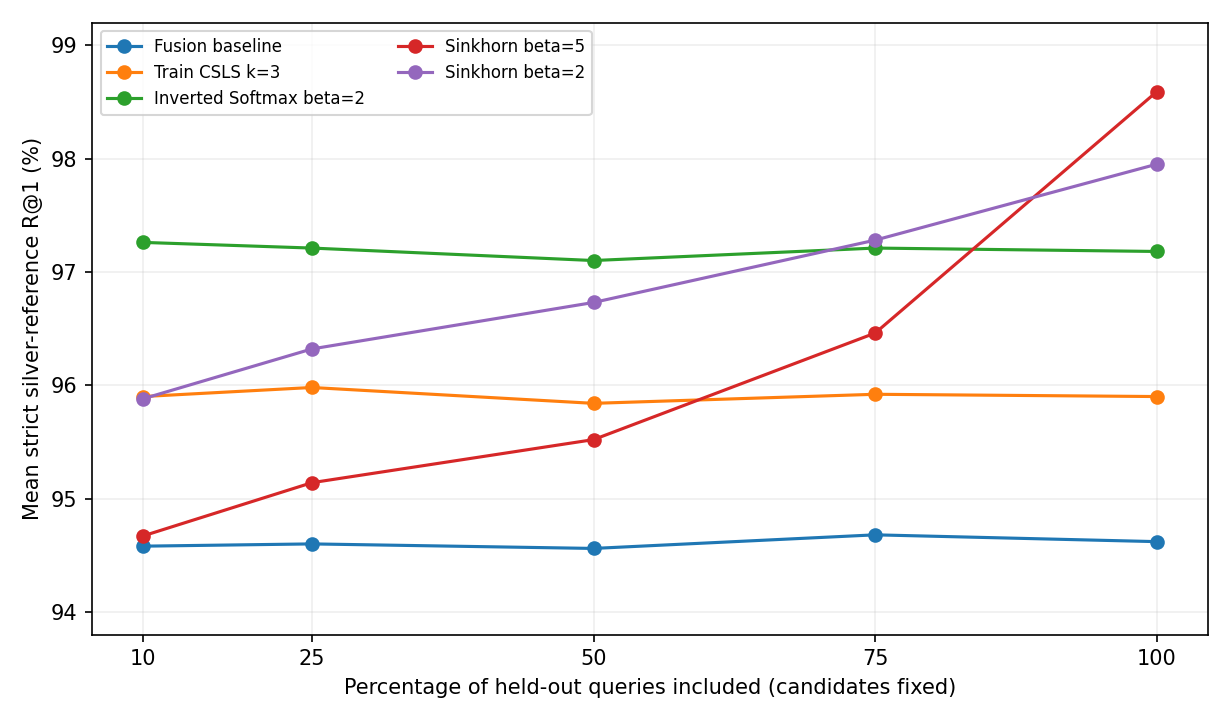
\includegraphics[width=0.85\textwidth]{query_subsampling.png}
\caption{Mean strict silver-reference R@1 as the fraction of held-out queries is reduced (candidates fixed at 780; 200 overlapping draws per partial fraction). The train-derived correction (k=3) is flat, whereas Sinkhorn at $\beta=5$ depends strongly on the batch.}
\label{fig:subsample}
\end{figure}

\paragraph{Mechanisms, not causal attribution.} Calibration makes top-1 assignments more evenly distributed (candidate-occupancy Gini 0.099 $\rightarrow$ 0.071), but the correlation between candidate density and the number of baseline top-1 errors assigned to a candidate is only about 0.02. This does not establish hubness as the source of all corrected errors. Since the neural component contributes in-sample E1 scores when estimating density from BA48 training queries, we also inspected retrospective out-of-fold E1$'$ controls. These use different encoders and improve their matched baselines but cannot substitute for a same-model out-of-fold experiment. No test in the present study adds genuinely unseen Vietnamese candidates, queries with no counterpart, or independent Bahnar-native source writing.

\section{Robustness and Validation Selection}\label{sec:robust}
\paragraph{Sensitivity to $k$ and rank metrics.} Table~\ref{tab:grid} shows that every $k$ from 1 to 10 improves on the 739/781 baseline (749--752 correct, exact McNemar $p$ between 0.001 and 0.031), so the result does not hinge on the pre-specified $k=3$; these are post hoc comparisons of one method family without multiplicity correction. The correction mainly moves queries into first place: R@5 rises from 762 to 766 and R@10 from 766 to 768 of 781, and MRR from 0.9600 to 0.9690 ($k=3$).

\paragraph{Per-family consistency.} Ten of the 20 test families gain, eight are unchanged and two lose (per-family counts are in the released analysis files). The two losing families lose two and one queries; the largest gain is three queries in a single 88-sentence family. With 20 families the cluster bootstrap interval is wide.

\paragraph{Validation replication.} The validation split (768 queries and candidates, 18 families) was scored with the same frozen pipeline before the test comparison, with the density term estimated from the same training queries. Table~\ref{tab:valid} shows the same direction on validation for the three values of $k$ examined there. Validation also chose the encoder checkpoint, so the validation baseline is itself slightly optimistic, and this split is not a clean replication.

\begin{table}[t]
\centering\small
\caption{Validation split (768 queries): same pipeline and training-query density term. Baseline 725/768.}
\label{tab:valid}
\begin{tabular}{rrrrc}
\toprule
$k$ & Correct & Fix/break & $p$ & 95\% interval (points) \\
\midrule
3 & 734 & 15/6 & 0.078 & $[+0.13,+2.07]$ \\
5 & 735 & 15/5 & 0.041 & $[+0.17,+2.30]$ \\
10 & 737 & 15/3 & 0.0075 & $[+0.43,+2.52]$ \\
\bottomrule
\end{tabular}
\end{table}

\paragraph{Validation-selected settings.} We also scored the 3,327 training queries against the 768 validation candidates (the lexical scores reproduce the archived validation matrices exactly) and applied the same train-derived rules there. Validation R@1 (baseline 725/768) for the train-derived correction rises from 730 at $k=1$ through 734 ($k=3$) and 735 ($k=5$) to 737 at $k=10$, and is 727, 731, \textbf{736}, 727 and 722 for Inverted Softmax at $\beta=0.5,1,2,5,10$. Selecting the best setting of each family on validation alone gives $k=10$ and $\beta=2$; applied once to the test, they give 752/781 (+14/$-$1, $p=0.001$, family-bootstrap interval $[+0.59,+2.76]$ points) and 759/781 (+20/$-$0, $p<0.001$); the locked primary contrast nevertheless remains $k=3$. The validation curve has the same peak at $\beta=2$ as the test curve, which supports the pattern in Table~\ref{tab:grid} as a property of the method and not of the test sample. Two limits remain: Inverted Softmax and the $\beta$ grid were first examined after test access, so the choice of candidate methods is not blind, and the transductive Sinkhorn results were not validated because its original marginal specification could not be recovered.

\section{Native-Speaker Spot Check}\label{sec:human}
This check was added after the primary result was frozen; it is not part of the locked protocol. Two Bahnar native speakers who agreed to take part labelled 88 items independently, each on a separate copy of one form: 18 queries on which the fixed baseline and the corrected system chose different candidates (14 counted as fixes and four as regressions by the silver reference), 60 randomly drawn non-discordant pairs, and 10 deliberately mismatched attention pairs. For the discordant queries, the two candidates were shown in a random order without indication of which system produced them, and each was labelled VALID, PARTIAL, INVALID or UNCERTAIN; controls were labelled YES, NO or UNCERTAIN. Reviewers could consult the source PDF but were told to judge the sentence pair itself.

\paragraph{Agreement.} The two reviewers gave the same label on all 88 items (Wilson 95\% lower bound 0.96). Their free-text reconstructions of the ten attention pairs differ (mean token-overlap $F_1$ 0.76), and their confidence scores differ on 7 of 88 items. The labels are easy for most items, so almost no label varies; we therefore report raw agreement and no chance-corrected statistic, and no third-party adjudication was needed.

\paragraph{Discordant pairs.} The silver reference was judged usable (VALID or PARTIAL) for 17 of the 18 queries (Wilson 95\% interval 0.74--0.99). Of the 14 queries counted as fixes, 13 were confirmed (corrected candidate VALID, baseline INVALID); one was judged the other way. Of the four counted as regressions, two were confirmed (corrected INVALID, baseline VALID) and two had a PARTIAL corrected candidate. Counting only VALID as correct, the net gain on these 18 queries is $13-5=+8$; counting VALID and PARTIAL as correct it is $13-3=+10$, equal to the silver count (Table~\ref{tab:human}).

\begin{table}[t]
\centering\small
\caption{Reviewer-confirmed outcomes on the 18 discordant queries (both reviewers gave identical labels). Strict counts only VALID as correct; lenient counts VALID and PARTIAL.}
\label{tab:human}
\begin{tabular}{lrrr}
\toprule
 & Silver & Strict & Lenient \\
\midrule
Corrected system better & 14 & 13 & 13 \\
Baseline better & 4 & 5 & 3 \\
Tie / not decisive & 0 & 0 & 2 \\
\midrule
Net gain on 18 queries & +10 & +8 & +10 \\
\bottomrule
\end{tabular}
\end{table}

\paragraph{Controls.} Both reviewers marked all 60 random non-discordant pairs as equivalent (Wilson lower bound 0.94) and all 10 mismatched attention pairs as not equivalent. These checks suggest that the silver labels are mostly sound on this sample; they do not estimate label error on the full 781-query test set, and 60 pairs cannot rule out an error rate of several percent.

\section{Practical Guidance and Conclusion}
\paragraph{What the evidence supports.} (i) If queries arrive individually against a fixed index, estimate candidate density from training queries: a train-derived CSLS-style or Inverted Softmax correction gave a small but consistent gain here and did not depend on batch size. (ii) Do not take a transductive normalization's full-batch figure as the expected deployed accuracy: Sinkhorn lost 3.9 points when only 10\% of the queries were present. (iii) Choose the temperature or $k$ on validation: validation picked $\beta=2$ and the test agreed, but the gain disappears at $\beta=5$.

\paragraph{Conclusion.} We isolated an information distinction within Bahnar--Vietnamese sentence retrieval: a CSLS-style correction can estimate candidate density from training queries without the unlabeled evaluation batch. On a fixed, silver-labelled benchmark, the internally pre-specified correction raised strict R@1 from 739/781 to 749/781; the paired gain is modest, cluster uncertainty rests on 20 families, and a blinded native-speaker check supports the labels on a small sample. A validation-selected Inverted Softmax and a transductive Sinkhorn variant score higher, but the first was added after test access and the second is sensitive to batch assumptions and unrecoverable provenance. Next steps require a larger adjudicated gold set, a new held-out collection and deployment-like index changes.

\section{Limitations}\label{sec:limitations}
\paragraph{Silver-label validity and small effect.} BA48 alignment is automated, and no complete, independently adjudicated Bahnar--Vietnamese gold set exists for this experiment. The primary net gain is only ten queries; it may be sensitive to a few incorrect references. A post hoc blinded check by two Bahnar native speakers (Section~\ref{sec:human}) covers only 18 discordant pairs and 60 controls; the reviewers agreed on every label, but the sample is small and was not part of the locked protocol, so it supports rather than establishes the validity of the silver labels. Reviewer credentials rest on self-report. Strict R@1 ignores multiple plausible translations. A larger native-speaker, multi-positive evaluation is a priority \emph{before} stronger semantic retrieval claims.

\paragraph{Population, pool and inference conditions.} One journalism-derived, largely translationese corpus, 781/780 fixed test pool and 20 graph-derived families do not establish performance across dialects, publishers, domains, or open-world retrieval. Family-cluster bootstrap assumes that resampling the observed clusters is informative; McNemar's exact query-level calculation does not accommodate within-family dependence. The test pool resembles one-to-one matching, a favorable regime for balancing methods; no unseen-index distractors or absent-counterpart queries were evaluated.

\paragraph{Reproducibility and exploratory selection.} Lexical scoring and frozen metric calculations were independently reconstructed, while E1 neural inference used archived matrices; an exact optimizer, software environment and original PDF-to-sentence aligner were not recovered. Historical source provenance is only partially traced. Test-time $\beta$ comparisons, IBM1 addition, out-of-fold controls and subsampling were all analyzed post-hoc. Original Sinkhorn row/column marginal settings cannot be fully attributed to their original run; the reported 770/781 is not an independently reproduced gold-metric result. Candidate density is estimated from training queries already seen by E1; its score-distribution implications remain incompletely isolated.

\section{Ethics and Data Availability}
The Bahnar source PDFs were publicly accessible to the operator's archival audit (170 logged URLs; 169 recorded SHA strings), but only 48 machine-extracted production-imprint candidates were detected and \emph{none} was visually adjudicated as a definitive per-issue masthead. Availability on a website does not itself determine permission to redistribute entire PDFs or text. The study is based on internal noncommercial research copies, with URLs and source hashes retained where available. Code, split identifiers, score-level metadata and non-textual audit summaries can be prepared separately; redistribution of source text or checkpoints remains subject to provenance and applicable permissions. The two reviewers agreed to take part (recorded on their forms), are not identified in the manuscript, and used only text already published by the newspaper; the check involved no personal data beyond the reviewers' self-reported language background.

\paragraph{Availability.} Code, split and query identifiers, hashes, per-query results for the baseline and corrected systems, and the anonymized reviewer labels (without newspaper text) are released at \repourl. Text and model checkpoints are not redistributed.

\bibliographystyle{splncs04}
\bibliography{references}
\appendix
\section{Sensitivity Notes}\label{app:explore}
The Sinkhorn figures in Section~\ref{sec:diagnostics} come from an archived 10-iteration, alternating row/column procedure whose exact marginal orientation was not recovered; retrospective reconstructions give identical top-1 counts across the variants we tried, but the 770/781 value is not an independently reproduced result. Query-fraction means (fusion / $k=3$ / Inv.\ $\beta=2$ / Sinkhorn $\beta=5$) are, in \%: 100\%: 94.62/95.90/97.18/98.59; 50\%: 94.56/95.84/97.10/95.52; 10\%: 94.58/95.90/97.26/94.67 (200 overlapping draws per partial fraction; all grid points and the full temperature scan were chosen after test access).

\paragraph{Neural training-score sensitivity.} E1 was adapted to the same 3,327 training pairs that also serve as density-reference queries. Post hoc five-fold, family-held-out E1$'$ models improved their own baselines by 13--21 queries at $k=3$, but E1$'$ differs appreciably from E1, so this cannot show the absence of an in-sample effect; a same-model cross-fitted reference would be needed.

\section{Per-Family Results}\label{app:family}
Table~\ref{tab:family} gives strict R@1 counts per document family for the pre-specified $k=3$ correction (families anonymized, ordered by size): ten improve, eight are unchanged and two decline.
\begin{table}[h]
\centering\scriptsize
\caption{Fusion and $k=3$ correct counts per held-out family.}
\label{tab:family}
\begin{tabular}{lrrrr|lrrrr}
\toprule
Fam. & $n$ & Fus. & $k=3$ & Net & Fam. & $n$ & Fus. & $k=3$ & Net \\
\midrule
F01&92&87&85&-2 & F11&31&30&30&+0 \\
F02&88&84&87&+3 & F12&31&31&30&-1 \\
F03&64&61&61&+0 & F13&31&29&30&+1 \\
F04&54&52&53&+1 & F14&31&30&30&+0 \\
F05&37&35&36&+1 & F15&30&25&26&+1 \\
F06&35&35&35&+0 & F16&29&27&27&+0 \\
F07&34&32&33&+1 & F17&26&26&26&+0 \\
F08&33&31&32&+1 & F18&25&22&23&+1 \\
F09&33&30&31&+1 & F19&23&21&21&+0 \\
F10&33&30&32&+2 & F20&21&21&21&+0 \\
\bottomrule
\end{tabular}
\end{table}

\section{IBM1 Same-Pool Baseline}\label{app:ibm1}
The publicly selected IBM1 symmetric configuration of Nguyen et al.~\cite{nguyen2026parallelretrieval} was run in a new, explicitly retrospective fit on our 55,324 historical pairs. It does not reuse the external study's model weights or its 46,736-pair split. We trained forward and backward co-occurrence-initialized translation tables for five EM iterations and scored all 781$\times$780 pairs, preserving the single shared Vietnamese gold candidate. Query/candidate IDs were joined to the frozen score matrices. Table~\ref{tab:ibm1} uses tie-conservative strict ranks and full-pool MRR throughout.
\begin{table}[h]
\centering\small
\caption{Within-BA48 comparison, including post-hoc IBM1. Metrics share identical candidate IDs.}
\label{tab:ibm1}

\begin{tabular}{lrrrr}
\toprule
System & R@1 & R@5 & R@10 & MRR \\
\midrule
IBM1 forward & .3764 & .5211 & .5762 & .4467 \\
IBM1 symmetric & .5186 & .6261 & .6748 & .5701 \\
Dice & .8143 & .9104 & .9321 & .8565 \\
Char TF--IDF & .8131 & .8758 & .8937 & .8427 \\
E1 & .8131 & .9052 & .9296 & .8578 \\
Fusion & .9462 & .9757 & .9808 & .9600 \\
Fusion + $k=3$ & .9590 & .9808 & .9834 & .9690 \\
\bottomrule
\end{tabular}
\end{table}

IBM1 symmetric fixes nine silver-reference errors of the corrected fusion but loses 353 queries it retrieves correctly.

\section{Cross-Corpus Overlap and Decontamination Audit}\label{app:corpus}
\paragraph{Method.} We cross-linked BA48's 5,094-row registry, the 55,324-pair historical dataset and the checksum-verified 2,001-query external test with exact rules (NFC/casefold, punctuation-insensitive, accent-folded) on whole pairs and single sides, plus same-record near-duplicate screening at 90\% and 95\% character similarity. Counts are of external queries matching at least one historical record and cannot be summed across categories.
\begin{table}[h]
\centering\small
\caption{Post-hoc overlap of the 2,001 external queries with the historical pairs. Exact one-sided sets overlap.}
\label{tab:corpus}

\begin{tabular}{lr}
\toprule
Rule & Queries matching historical \\
\midrule
Strict exact bilingual & 67 \\
Strict exact Bahnar side & 118 \\
Strict exact Vietnamese side & 541 \\
Punctuation-insensitive bilingual exact & 284 \\
Bilingual punctuation exact OR near $\geq90\%$ & 356 \\
\bottomrule
\end{tabular}
\end{table}

No bilingual or single-side exact matches were observed between any BA48 split and the historical set under the three normalizations, or between BA48's training reservoir, validation and test; same-record two-sided near $\geq90\%$ screening also returned zero between the external test and BA48. The external overlap with historical does \emph{not} imply leakage in the other study's own train/test split. The E1 auxiliary dataset comprises 50,283 of the historical pairs but its exact membership manifest was not available; consequently historical overlap cannot all be assigned to E1. Conditional query-level bounds, using the known historical exclusion partition, are 0--37 for strict-exact bilingual matches and 201--243 for punctuation-insensitive bilingual matches; these are not independently verified exact membership counts. The original 53,610-pair E1 training manifest is required to resolve them.

\section{Archival Provenance and Reproducibility}\label{app:provenance}
The access log has 170 PDF URL records, 169 with a syntactically valid recorded SHA-256 (hashes checked for syntax and URL linkage, not re-hashed); one 32-page file failed parsing (four BA48 pairs). Forty-eight page snippets contain production-imprint patterns that do not establish masthead identity without page images. The font tables, silver alignment procedure, E1 optimizer and exact dependency versions were not fully recovered, so end-to-end encoder reproduction remains outstanding.

\end{document}
